\section{Bài 3}
Trong bài này chúng ta sẽ xem xét bài toán dóng hàng
toàn cục 2 chuỗi DNA sử dụng phương pháp quy hoạch động 
với giải thuật Needleman-Wunsch.

\subsection{Bài toán dòng hàng toàn cục}
Có nhiều cách để phát biểu bài toán dóng hàng trình tự 
(cho DNA, RNA hoặc 2 chuỗi kí tự). Hãy cùng điểm qua vài khái niệm.

\begin{itemize}
    \item Dóng hàng trình tự: là một cách sắp xếp trình tự của DNA,
    RNA hoặc protein để xác định các vùng giống nhau có thể là
    hệ quả của mối quan hệ chức năng, cấu trúc hoặc tiến hóa giữa
    các trình tự.
    \item Một cách dóng hàng của 2 chuỗi được thiết lập bằng cách thêm
    các khoảng trống (dấu cách) vào các vị trí bất kì trên 2 chuỗi này
    để chúng có cùng độ dài và không có 2 khoảng trống nào có cùng vị trí 
    trên 2 chuỗi
    \item Chuỗi con chung dài nhất (longest common subsequence, LCS):
    là chuỗi trình tự chứa nhiều kí tự giống nhau nhất của hai hay
    nhiều chuỗi.
\end{itemize}
Ví dụ một cách dóng hàng với 2 chuỗi S (\lstinline{interestingly}) 
và T (\lstinline{bioinformatics}) như sau
\begin{center}
    \lstinline{-i--nterestingly} \\
    \lstinline{bioinformatics--}
\end{center}

Một cách tổng quát, chúng ta có thể chấm điểm cho mỗi cặp kí tự được dóng hàng.
Gọi $\Sigma$ là tập các kí tự và "-" là kí tự đặc biệt kí hiệu cho dấu cách. 
Sự tương tự của các cặp kí tự trong 2 chuỗi có thể được biểu diễn thông qua 
một ma trận $\delta$ mà $\delta(x,y)$ là điểm của cặp $x$ và $y$ với 
$x, y \in \Sigma \cup \{-\}$. \\
Bài toán dóng hàng toàn cục có thể mô hình hóa bằng cách tìm một cách dóng hàng A
nào đó để cực đại $\sum_{\{x, y \} \in A} \delta(x,y)$. Cách dóng hàng này được
gọi là cách tối ưu (\textit{optimal alignment}). \\
Khi một cặp kí tự được sắp xếp và giống nhau, liên hệ giữa chúng
 được gọi là \textit{match}, ngược
lại gọi là \textit{mismatch}. Khi dấu cách được thêm vào chuỗi thứ nhất mối liên hệ 
là \textit{insert}, khi được thêm vào chuỗi thứ 2 thì được gọi là \textit{delete}. \\
Trong ví dụ trên chúng ta có 5 \textit{matches}, 6 \textit{mismatchs}, 3 \textit{inserts}
và 2 \textit{deletes}.

Chúng ta cùng xem xét một ví dụ về dóng hàng toàn cục. Xét ma trận điểm cho tập 
$\{-, A, C, G, T\}$ với $\delta(x, y) = 2, -1, -1, -1$ lần lượt cho match, mismatch, 
delete và insert. Xét 2 chuỗi DNA $S = ACAATCC$ và $T = AGCATGC$, một cách dóng hàng
khả dĩ như sau:
\begin{center}
    \lstinline{S = A-CAATCC} \\
    \lstinline{T = AGCA-TGC}
\end{center}
Cách dóng hàng trên có 5 matches, 1 mismatch, 1 insert và 1 delete. Vậy điểm tương tự của 
cách dòng hàng này là 7. Có thể kiểm tra được đây là điểm cực đại thế nên cách dóng hàng
này là một cách tối ưu. Cần chú ý là có thể có nhiều hơn một cách dóng hàng tối ưu. 
Ví dụ 1 cách khác cũng trả về điểm tương tự cực đại.
\begin{center}
    \lstinline{S = A-CAATCC} \\
    \lstinline{T = AGC-ATGC}
\end{center}

\begin{figure}[H] % places figure environment here   
    \centering % Centers Graphic
    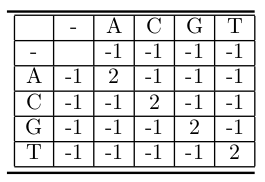
\includegraphics[width=0.3\textwidth]{./assets/score_matrix.png} 
    \caption{Ví dụ ma trận điểm tương tự} % Creates caption underneath graph
\end{figure}

\subsection{Giải thuật Needleman-Wunsch}
\subsubsection{Giải thuật}
Xét 2 chuỗi kí tự $S[1...n]$ và $T[1...m]$. Để tìm cách dóng hàng toàn cục tối ưu cho 
bài toán này chúng ta có thể nghĩ tới giải thuật vét cạn bằng cách sinh ra mọi cách 
dóng hàng và tìm xem cách nào có điểm cao nhất. Tuy nhiên cách tiếp cận này có thời
gian tính toán theo hàm mũ. Trong phần này, chúng ta sẽ xem xét một giải thuật hiệu quả
áp dụng \textit{quy hoạch đông} có tên là \textit{Needleman-Wunsch}. \\
Chúng ta thiết kế một hàm đệ quy (công thức truy hồi) $V(i,j)$ với 2 trường hợp: (1) $i = 0$ 
hoặc $j = 0$ và (2) cả $i > 0$ và $j > 0$. \\
Với trường hợp (1) khi $i = 0$ hoặc $j = 0$ chúng ta dóng hàng chuỗi bằng 1 chuỗi rỗng.
Hay nói cách khác là ta chỉ cần thêm hoặc xóa kí tự. Chúng ta có các phương trình:
\begin{equation}
    \begin{aligned}
        V(0, 0) &= 0 & \\
        V(0, j) &= V(0, j - 1) + \delta(-, T[j]) && \text{thêm j lần} \\
        V(i, 0) &= V(i -1, 0) + \delta(S[i], -) && \text{xóa i lần} 
    \end{aligned}
\end{equation}
Với trường hợp (2) khi cả $i > 0$ và $j > 0$, ta thấy rằng với một cách dóng hàng nào đó
của chuỗi $S[1...i]$ và $T[1...j]$ cặp kí tự cuối cùng phải thuộc 1 trong 3 loại 
match/mismatch (cả 2 đều là kí tự), insert hoặc delete. Để thu được điểm tối ưu ta chọn 
cách có điểm cực đại trong 3 trường hợp trên. Nghĩa là:
\begin{equation}
    V(i, j) = \max 
    \begin{cases}
        V(i - 1, j - 1) + \delta(S[i], T[j]) & \text{match/mismatch} \\
        V(i - 1, j) + \delta(S[i], -) & \text{delete} \\
        V(i, j - 1) + \delta(-, T[j]) & \text{insert} \\
    \end{cases}
\end{equation}
Điểm dóng hàng tối ưu của $[1...n]$ và $T[1...m]$ là $V(n,m)$. Điểm này có thể được tính bằng
cách điền đầy từng hàng vào bảng $V(1...n, 1...m)$ bằng các công thức truy hồi trên.

\begin{figure}[H] % places figure environment here   
    \centering % Centers Graphic
    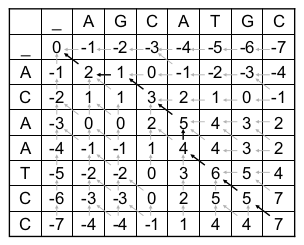
\includegraphics[width=0.4\textwidth]{./assets/dp.png} 
    \caption{Bảng điểm dóng hàng 2 chuỗi $S = ACAATCC$ và $T = AGCATGC$
    bằng giải thuật quy hoạch động Needleman-Wunsch} % Creates caption underneath graph
    \label{fig:dp_track}
\end{figure}

Hình trên là bảng $V$ cho 2 chuỗi $S = ACAATCC$ và $T = AGCATGC$.
Chúng ta có thể tính lần lượt giá trị của các ô trong bảng, ví dụ $V(1, 1)$ là giá trị 
lớn nhất trong tập $\{0+2, -1-1, -1-1\}$. Sau khi điền đầy các ô ta có $V(7,7) = 7$ là 
giá trị của ô dưới cùng bên phải hay chính là điểm của cách dóng hàng tối ưu.

Để tìm ngược lại cách dóng hàng tối ưu, với mỗi ô trong bảng ta vẽ các mũi tên để biểu 
diễn sự tương quan giữa các cặp. Ta vẽ mũi tên chéo, ngang và dọc lần lượt cho các trường
hợp match, insert và delete. Ví dụ giá trị tại $V(1,1)$ thu được bởi $V(0,0) + 2$, chúng 
ta vẽ 1 mũi tên chéo. Với ô $V(3,2)$, có 2 cách có giá trị điểm bằng điểm lớn nhất nên 
ta vẽ cả 2 mũi tên chéo và dọc. Để thu được cách dóng hàng tối ưu ta cần quay lui từ ô 
$V(7,7)$ về ô $V(0,0)$. Nếu mũi tên là chéo, 2 kí tự được dóng hàng. Với mũi tên ngang và
dọc thì lần lượt là delete và insert. Ta thu được đường quay lui là đường mũi tên in đậm 
trong hình \ref{fig:dp_track} theo đường $7 \to 5 \to 6 \to 4 \to 5 \to 3 \to 1 \to 0$.
Tương ứng ta thu được cách dóng hàng tối ưu:

\begin{center}
    \lstinline{A-CAATCC} \\
    \lstinline{AGCA-TGC}
\end{center}

\subsubsection{Thời gian tính toán}
Như đã trình bày trong phần trước, thuật toán Needleman-Wunsch có thời gian tính toán là $O(nm)$
khi giải bài toán dóng hàng toàn cục do chúng ta cần điền vào toàn bộ các ô trong bảng điểm 
dòng hàng có kích thước $n \times m$

\subsection{Triển khai thuật toán}
Trong phần này chúng ta sẽ đưa ra mã giả cài đặt thuật toán Needleman-Wunsch để lập bảng điểm
dóng hàng và trình bày cách quay lui để đưa ra kết quả dóng hàng 2 chuỗi DNA. \\
Thay vì gọi là \textit{bảng} như phần trước, chung ta sẽ xây dựng một 
\textit{ma trận} $V$ gọi là ma trận \textit{score}.
Ở đây ta kí hiệu $v[i, j]$ là thành phần $v_{i,j}$ của ma trận $V$,
$s[i]$ là kí tự tại chỉ số $i$ của chuỗi $s$ (lưu ý chỉ số đánh từ $0$). \\
Trước hết là mã giả để  xây dựng ma trận $V$ hay nói cách khác là điền đầy 
bảng điểm dóng hàng của 2 chuỗi $s$ và $t$. \\

\begin{lstlisting}[style=algo]
    // alias for backtracking arrows
    left, up, dia = 1, 2, 3 

    // define score for characters status
    match, mismatch, insert, delete = 2, -1, -1, -1

    delta(a, b):
        // define score
        if a == b:
            return match
        if '-' == a:
            return insert
        if '-' == b:
            return delete
        return mismatch
    end

    node_score(s, t, node, i, j):
        // calculate score of node[i, j]
        score_match_mismatch = node[i-1, j-1] \
            + delta(s[i], t[j])
        score_delete = node[i-1, j] + delta(s[i], '-')
        score_insert = node[i, j-1] + delta(s[i], '-')
        return max([score_match_mismatch, 
                    score_delete, 
                    score_insert])
    end


    lsc(s, t):
        // fill the score table
        n = length of s
        m = length of t
        backtrack = zero matrix with size $(n+1) \times (m+1)$
        v = zero matrix with size $(n+1) \times (m+1)$
        s = '-' + s
        t = '-' + t

        for i from 0 to n:
            v[i, 0] = -i

        for j from 0 to m:
            v[0, j] = -j

        for i from 1 to n:
            for j from 0 to m:
                v[i, j] = node_score(s, t, v, i, j)
                if v[i, j] == v[i-1, j] + delta(s[i], '-'):
                    backtrack[i, j] = up
                elif v[i, j] == v[i, j-1] + delta('-', t[j]):
                    backtrack[i, j] = left
                else:
                    backtrack[i, j] = dia

        return v, backtrack
    end
\end{lstlisting}

Tiếp theo ta có mã giả cho quá trình quay lui để đưa ra kết quả dòng hàng
\begin{lstlisting}[style=algo]
    output(s, t, backtrack):
        // return 2 aligned sequences
        n = length of s
        m = length of t
        source, target = s, t
        i, j = n, m
        while i > 0 and j > 0:
            if backtrack[i, j] == left:
                inserting '-' to source at index $(j-1)$
                j = j - 1
                continue
            if backtrack[i, j] == up:
                inserting '-' to target at index $(i-1)$
                i = i - 1
                continue
            i = i - 1
            j = j - 1
        return source, target
    end
\end{lstlisting}

Cuối cùng là \href{https://github.com/batman0911/dma_homework/blob/master/hw_01/src/sequence.ipynb}{python code} 
cài đặt thuật toán.  